\documentclass{beamer}
\usepackage[utf8]{inputenc}
\usepackage[T1]{fontenc}
\usepackage{csquotes,lipsum}
\usepackage{listings}
\usepackage{xcolor}
\usepackage{dsfont}
\usepackage{multicol}
\usepackage[linesnumbered]{algorithm2e}


\definecolor{codegreen}{rgb}{0,0.6,0}
\definecolor{codegray}{rgb}{0.5,0.5,0.5}
\definecolor{codepurple}{rgb}{0.58,0,0.82}
\definecolor{backcolour}{rgb}{0.95,0.95,0.92}

\lstdefinestyle{mystyle}{
    backgroundcolor=\color{backcolour},
    commentstyle=\color{codegreen},
    keywordstyle=\color{magenta},
    numberstyle=\tiny\color{codegray},
    stringstyle=\color{codepurple},
    basicstyle=\ttfamily\footnotesize,
    breakatwhitespace=false,
    breaklines=true,
    captionpos=b,
    keepspaces=true,
    numbers=left,
    numbersep=5pt,
    showspaces=false,
    showstringspaces=false,
    showtabs=false,
    tabsize=2
}
\lstset{style=mystyle}


\renewcommand{\mkblockquote}[4]{#1#2\par\hfill#4#3}


\title{5GEN: A tool to generate 5G infrastructure graphs}
\date{30\textsuperscript{th} October, 2019}
\author{Jorge Martín Pérez}

\usetheme{uc3m}

\begin{document}

\begin{frame}
\titlepage
\end{frame}

\setcounter{framenumber}{0}


\begin{frame}{Table of contents}
    \tableofcontents
\end{frame}

\section{Introduction}
\begin{frame}{What is 5GEN?}
     A \textbf{R} package\footnote{\scriptsize \url{https://github.com/MartinPJorge/mec-generator/tree/5g-infra-gen}} to generate 5G network infrastructure graphs.

    \begin{figure}
        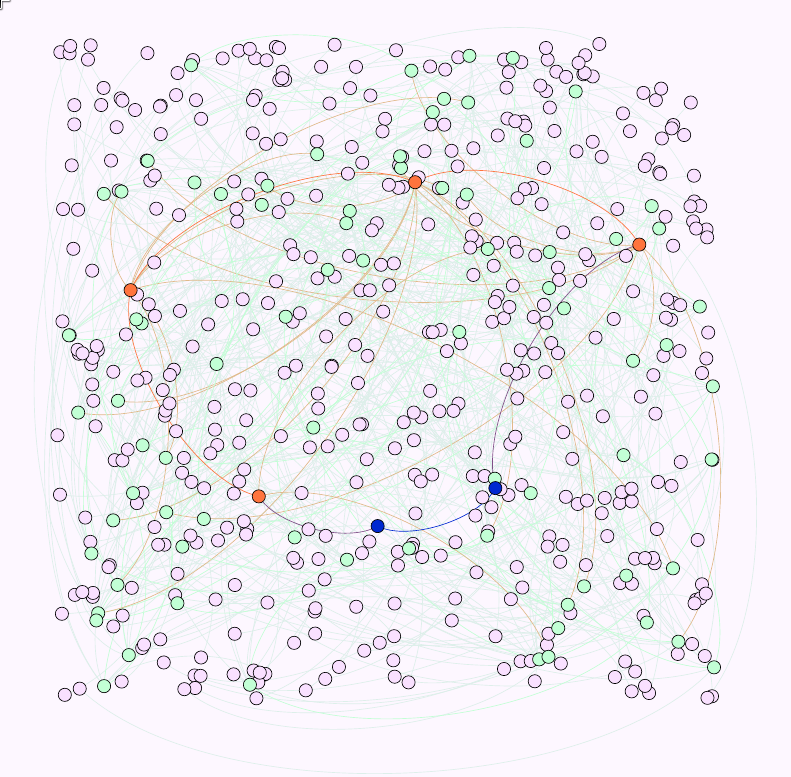
\includegraphics[width=0.5\textwidth]{img/infra-graphs.png}
        \caption{A graph generated by 5GEN.}
        \label{fig:5gen-graph}
    \end{figure}
\end{frame}



\begin{frame}{What do 5GEN graphs represent?}
    \begin{columns}[T]
        \begin{column}{.48\textwidth}
            \vspace{2.5em}
            The network infrastructure \textbf{up to the core}.
            \begin{itemize}
                \item Active Antenna Units (AAUs);
                \item M1, M2 and M3 switches;
                \item Servers; and
                \item Fog nodes
            \end{itemize}
        \end{column}
        \begin{column}{.48\textwidth}
            \begin{figure}
                \includegraphics[width=0.8\textwidth]{img/infra-elements.pdf}
                \caption{Some 5GEN graph components}
            \end{figure}
        \end{column}
    \end{columns}
\end{frame}

\section{Motivation}
\begin{frame}{Why we needed 5GEN?}
    To validate solutions for the Virtual Network Embedding (VNE) problem:
    \begin{center}
        \begin{minipage}{0.6\textwidth}
            \begin{block}{}
                \blockquote[\cite{fischer2013virtual}][]{The problem of embedding virtual networks in a substrate network}
            \end{block}
        \end{minipage}
    \end{center}
    \begin{figure}
        \only<1>{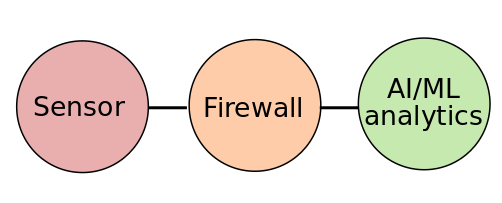
\includegraphics[width=0.8\textwidth]{img/vne-sfc.pdf}}
        \only<2>{\includegraphics[width=0.8\textwidth]{img/vne-infra.pdf}}
        \only<3>{\includegraphics[width=0.8\textwidth]{img/vne-solution.pdf}}
        \caption{VNE example}
        \label{fig:vne-example}
    \end{figure}
\end{frame}


\section{Generating the graphs}
\begin{frame}{Before generating the graphs}
    Open questions:
    \begin{itemize}
        \item AAUs per switch?;
        \item Switches per ``level''?;
        \item Interconnections; and
            \begin{itemize}
                \item Hierarchical;
                \item Ring; and
                \item Redundancy;
            \end{itemize}
        \item Traffic rates;
    \end{itemize}
\end{frame}

\begin{frame}{Reference topology}
    Use analysis in \cite{luca-5g-qos}, based on ITU-T study group analysis \cite{itu}
    \begin{figure}
        \includegraphics[width=\textwidth]{img/infra-reference-fog.pdf}
        \caption{5GEN reference topologies}
    \end{figure}
\end{frame}


\begin{frame}{Topology generation steps}
    \begin{enumerate}
        \item Specify AAUs' locations;
        \item Calculate required M1 switches and access rings;
        \item Calculate required M2 switches and aggregation rings;
        \item Derive how many M3 switches; and
        \item Attach user-defined elements:
            \begin{itemize}
                \item Fog devices;
                \item Servers \& where (M1, M2, M3);
            \end{itemize}
    \end{enumerate}
\end{frame}


\begin{frame}[fragile]{Specify AAUs' locations}
    5GEN assumes a set of AAUs distributed across an area, e.g., Granada.

    \begin{figure}
        \includegraphics[width=0.6\textwidth]{img/granada-map-with-aaus.pdf}
        \caption{Location of an AAU in Granada}
    \end{figure}


    \begin{lstlisting}[language=R]
granadaCells[1,]$lat; granadaCells[1,]$lon
[1] 37.1716524
[2] -3.5932497\end{lstlisting}
\end{frame}



\begin{frame}{CSCN19 Granada AAUs CSV}
    CSV with AAUs locations at \url{https://github.com/MartinPJorge/cscn19/granada-cells.csv}
    \begin{itemize}
        \item 12 AAUs/km\textsuperscript{2}
        \item 10m repulsion radius
        \begin{equation}
            \mathbb{E}\left[ N(C) \right] := \int_C e^{-\int_{B(x,r)} \mathds{1}\left(\lambda(u) > \lambda(x) \right) \lambda(u) du} \lambda(x)\ dx
            \label{eq:inh-matern2-avg}
        \end{equation}
    \end{itemize}

    \begin{figure}
        \includegraphics[width=0.6\textwidth]{img/granda-map-csv-aaus.pdf}
        \caption{AAUs generated with a Matérn II PPP \cite{repulsion}}
    \end{figure}
\end{frame}




\begin{frame}{5GEN algorithm}


    \begin{columns}[T]
        \begin{column}{0.4\textwidth}

            \scalebox{0.4}{
            \begin{minipage}{2.3\textwidth}


                \begin{algorithm}[H]
                 \KwData{AAUs}
                 \KwResult{access and aggregation graph}
                 levels = [AAUs, access, aggregation]\;
                 distances = [10km, 20km, 40km]\;
                 \ForEach{($l$, $d$) in (levels, distance)}{
                     \begin{equation*}
                         N=\begin{cases}
                             AAUs, &  \text{if}\ l=\text{AAUs}\\
                             M1, &    \text{if}\ l=access\\
                             M2, &    \text{if}\ l=aggregation\\
                         \end{cases}
                     \end{equation*}

                     $H$ = hierarchical\_clustering($N$)\;\label{alg:clustering}
                     $C$ = cut\_dendrogram($H$, $d$)\;\label{alg:cut-dendrogram}
                     $R = \cup_{C'\in C} \left\{ \left\{ C'_{i+6j} \right\}_{i=0}^{\min \{C'-1-6j,5\}} \right\}_{j=0}^{\lfloor C'/6 \rfloor}$\;\label{alg:split-in-6}
                     \eIf{$l=\text{AAUs}$}{
                         \For{$R_j\in R$}{
                             $\text{M1}_n=\min_{\text{M1}}\sum_{r\in R_j} \text{Vicenty}\left(\text{M1},r\right)$\;
                             connect$\left( r, \text{M1}_n \right),\ \forall r\in R_j$\;
                         }
                     }{
                     connect$\left( r_i, r_{i+1\mod 6} \right),\ \forall r_i\in R_j,\ \forall R_j\in R$\;\label{alg:connect-ring}
                        $g = 4\ \text{if}\ l=\text{M1}\ \text{else}\ 2$\;
                        $G=\left\{ \left\{ R_{i+gj} \right\}_{i=0}^{\min \{R-1-gj,g-1\}} \right\}_{j=0}^{\lfloor R/g \rfloor }$\;\label{alg:group-ring}
                        \For{$G_i\in G$}{
                            upper$=$M2 if $l=$M1 else M3\;
                            connect'$\left( R, \text{upper} \right),\ \forall R \in G_i$\;\label{alg:ring-up}
                        }
                     }
                 }
                 \caption{build5GScenario}
                 \label{alg:build-5g-scenario}
                \end{algorithm}

            \end{minipage}
            }
        \end{column}
        \begin{column}{0.58\textwidth}
            \vspace{3em}
            It executes clustering to:
            \begin{itemize}
                \item Group AAUs;
                \item Create the access ring; and
                \item Create aggregation ring.
            \end{itemize}
            \vspace{0.5em}

            R package \textbf{mecgen} performs everything underneath inside function \textbf{build5GScenario}.
        \end{column}
    \end{columns}
\end{frame}




\begin{frame}{AAUs assignment to M1s}
    \only<1>{\begin{columns}[T]
        \begin{column}{0.48\textwidth}
            \begin{minipage}{1.5\textwidth}
            \begin{algorithm}[H]
                                 $H$ = hierarchical\_clustering($N$)\;\label{alg:clustering}
                                 $C$ = cut\_dendrogram($H$, $d$)\;\label{alg:cut-dendrogram}
                                 $R = \cup_{C'\in C} \left\{ \left\{ C'_{i+6j} \right\}_{i=0}^{\min \{C'-1-6j,5\}} \right\}_{j=0}^{\lfloor C'/6 \rfloor}$\;\label{alg:split-in-6}
                                 \For{$R_j\in R$}{
                                     $\text{M1}_n=\min_{\text{M1}}\sum_{r\in R_j} \text{Vicenty}\left(\text{M1},r\right)$\;
                                     connect$\left( r, \text{M1}_n \right),\ \forall r\in R_j$\;
                                 }
            \end{algorithm}
            \end{minipage}
        \end{column}
    \end{columns}}


    \only<2->{\begin{columns}[T]
        \begin{column}{0.38\textwidth}
            \scalebox{0.6}{
            \begin{minipage}{1.6\textwidth}
            \begin{algorithm}[H]
                                 $H$ = hierarchical\_clustering($N$)\;\label{alg:clustering}
                                 $C$ = cut\_dendrogram($H$, $d$)\;\label{alg:cut-dendrogram}
                                 $R = \cup_{C'\in C} \left\{ \left\{ C'_{i+6j} \right\}_{i=0}^{\min \{C'-1-6j,5\}} \right\}_{j=0}^{\lfloor C'/6 \rfloor}$\;\label{alg:split-in-6}
                                 \For{$R_j\in R$}{
                                     $\text{M1}_n=\min_{\text{M1}}\sum_{r\in R_j} \text{Vicenty}\left(\text{M1},r\right)$\;
                                     connect$\left( r, \text{M1}_n \right),\ \forall r\in R_j$\;
                                 }
            \end{algorithm}
            \end{minipage}
            }
        \end{column}

        \begin{column}{0.6\textwidth}
            \only<2>{\begin{figure}
                \includegraphics[width=\textwidth]{img/granda-map-aaus-clustered.pdf}
                \caption{AAUs clustering representation\footnotemark}
            \end{figure}}
            \only<3>{\begin{figure}
                \includegraphics[width=\textwidth]{img/granda-map-aaus-clustered-m1s.pdf}
                \caption{AAUs clustering representation\footnotemark}
            \end{figure}}
        \end{column}
    \end{columns}
        \footnotetext[1]{6 AAUs per cluster, none of them left out}
    }
\end{frame}




\begin{frame}{Creating the access ring}
    \only<1>{\begin{columns}[T]
        \begin{column}{0.48\textwidth}
            \begin{minipage}{1.5\textwidth}
            \begin{algorithm}[H]
                                 $H$ = hierarchical\_clustering($N$)\;\label{alg:clustering}
                                 $C$ = cut\_dendrogram($H$, $d$)\;\label{alg:cut-dendrogram}
                                 $R = \cup_{C'\in C} \left\{ \left\{ C'_{i+6j} \right\}_{i=0}^{\min \{C'-1-6j,5\}} \right\}_{j=0}^{\lfloor C'/6 \rfloor}$\;\label{alg:split-in-6}
     connect$\left( r_i, r_{i+1\mod 6} \right),\ \forall r_i\in R_j,\ \forall R_j\in R$\;\label{alg:connect-ring}
            \end{algorithm}
            \end{minipage}
        \end{column}
    \end{columns}}


    \only<2->{\begin{columns}[T]
        \begin{column}{0.38\textwidth}
            \scalebox{0.6}{
            \begin{minipage}{1.9\textwidth}
                \vspace{5em}
            \begin{algorithm}[H]
                                 $H$ = hierarchical\_clustering($N$)\;\label{alg:clustering}
                                 $C$ = cut\_dendrogram($H$, $d$)\;\label{alg:cut-dendrogram}
                                 $R = \cup_{C'\in C} \left\{ \left\{ C'_{i+6j} \right\}_{i=0}^{\min \{C'-1-6j,5\}} \right\}_{j=0}^{\lfloor C'/6 \rfloor}$\;\label{alg:split-in-6}
     connect$\left( r_i, r_{i+1\mod 6} \right),\ \forall r_i\in R_j,\ \forall R_j\in R$\;\label{alg:connect-ring}
            \end{algorithm}
            \end{minipage}
            }
        \end{column}

        \begin{column}{0.6\textwidth}
            \begin{figure}
                \includegraphics[width=\textwidth]{img/granada-map-access-rings}
                \caption{Access rings representation}
            \end{figure}
        \end{column}
    \end{columns}
    }
\end{frame}








\begin{frame}{Assignment of access rings to M2s}
    \only<1>{\begin{columns}[T]
        \begin{column}{0.48\textwidth}
            \begin{minipage}{1.5\textwidth}
            \begin{algorithm}[H]
                                 $H$ = hierarchical\_clustering($N$)\;\label{alg:clustering}
                                 $C$ = cut\_dendrogram($H$, $d$)\;\label{alg:cut-dendrogram}
                                 $R = \cup_{C'\in C} \left\{ \left\{ C'_{i+6j} \right\}_{i=0}^{\min \{C'-1-6j,5\}} \right\}_{j=0}^{\lfloor C'/6 \rfloor}$\;\label{alg:split-in-6}
     connect$\left( r_i, r_{i+1\mod 6} \right),\ \forall r_i\in R_j,\ \forall R_j\in R$\;\label{alg:connect-ring}
        $g = 4\ \text{if}\ l=\text{M1}\ \text{else}\ 2$\;
        $G=\left\{ \left\{ R_{i+gj} \right\}_{i=0}^{\min \{R-1-gj,g-1\}} \right\}_{j=0}^{\lfloor R/g \rfloor }$\;\label{alg:group-ring}
        \For{$G_i\in G$}{
            upper$=$M2 if $l=$M1 else M3\;
            connect'$\left( R, \text{upper} \right),\ \forall R \in G_i$\;\label{alg:ring-up}
        }
            \end{algorithm}
            \end{minipage}
        \end{column}
    \end{columns}}


    \only<2->{\begin{columns}[T]
        \begin{column}{0.38\textwidth}
            \vspace{2em}
            \scalebox{0.6}{
            \begin{minipage}{2\textwidth}
            \begin{algorithm}[H]
                                 $H$ = hierarchical\_clustering($N$)\;\label{alg:clustering}
                                 $C$ = cut\_dendrogram($H$, $d$)\;\label{alg:cut-dendrogram}
                                 $R = \cup_{C'\in C} \left\{ \left\{ C'_{i+6j} \right\}_{i=0}^{\min \{C'-1-6j,5\}} \right\}_{j=0}^{\lfloor C'/6 \rfloor}$\;\label{alg:split-in-6}
     connect$\left( r_i, r_{i+1\mod 6} \right),\ \forall r_i\in R_j,\ \forall R_j\in R$\;\label{alg:connect-ring}
        $g = 4\ \text{if}\ l=\text{M1}\ \text{else}\ 2$\;
        $G=\left\{ \left\{ R_{i+gj} \right\}_{i=0}^{\min \{R-1-gj,g-1\}} \right\}_{j=0}^{\lfloor R/g \rfloor }$\;\label{alg:group-ring}
        \For{$G_i\in G$}{
            upper$=$M2 if $l=$M1 else M3\;
            connect'$\left( R, \text{upper} \right),\ \forall R \in G_i$\;\label{alg:ring-up}
        }

            \end{algorithm}
            \end{minipage}
            }
        \end{column}

        \begin{column}{0.6\textwidth}
            \begin{figure}
                \includegraphics[width=\textwidth]{img/granada-map-access-to-m2.pdf}
                \caption{M2 switch handling x4 access rings' traffic}
            \end{figure}
        \end{column}
    \end{columns}
    }
\end{frame}





\begin{frame}{Aggregation rings and M3s}
    \begin{columns}[T]
        \begin{column}{0.38\textwidth}
            \vspace{2em}
            \scalebox{0.6}{
            \begin{minipage}{2\textwidth}
            \begin{algorithm}[H]
                                 $H$ = hierarchical\_clustering($N$)\;\label{alg:clustering}
                                 $C$ = cut\_dendrogram($H$, $d$)\;\label{alg:cut-dendrogram}
                                 $R = \cup_{C'\in C} \left\{ \left\{ C'_{i+6j} \right\}_{i=0}^{\min \{C'-1-6j,5\}} \right\}_{j=0}^{\lfloor C'/6 \rfloor}$\;\label{alg:split-in-6}
     connect$\left( r_i, r_{i+1\mod 6} \right),\ \forall r_i\in R_j,\ \forall R_j\in R$\;\label{alg:connect-ring}
        $g = 4\ \text{if}\ l=\text{M1}\ \text{else}\ 2$\;
        $G=\left\{ \left\{ R_{i+gj} \right\}_{i=0}^{\min \{R-1-gj,g-1\}} \right\}_{j=0}^{\lfloor R/g \rfloor }$\;\label{alg:group-ring}
        \For{$G_i\in G$}{
            upper$=$M2 if $l=$M1 else M3\;
            connect'$\left( R, \text{upper} \right),\ \forall R \in G_i$\;\label{alg:ring-up}
        }

            \end{algorithm}
            \end{minipage}
            }
        \end{column}

        \begin{column}{0.6\textwidth}
            \begin{figure}
                \includegraphics[width=\textwidth]{img/granada-map-aggregation-rings.pdf}
                \caption{Aggregation rings' representation}
            \end{figure}
        \end{column}
    \end{columns}
\end{frame}



\begin{frame}[fragile]{How does \textbf{mecgen} deal with it?}
    Just invoke \textbf{build5GScenario} with AAUs' locations

    \begin{lstlisting}[language=R]
granadaCells <- read.csv('granada-cells.csv')
assocs <- build5GScenario(lats = granadaCells$lat,
                          lons = granadaCells$lon)\end{lstlisting}

    \textbf{assocs} contains dataframes with:
    \begin{itemize}
        \item AAUs to M1s;
        \item M1s to M1s;
        \item Access rings to M2;
        \item M2s to M2s; and
        \item Aggregation rings to M3s.
    \end{itemize}
\end{frame}


\begin{frame}[fragile]{Addition of compute nodes}
    E.g., add server nodes
    \begin{lstlisting}[language=R]
...
graph <- attachServers(nodes = graph$nodes,
                       links = graph$links,
                       numServers = 3,
                       bandwidth = 12,
                       bandwidthUnits = "Mbps",
                       distance = 0,
                       distanceUnits = "meter",
                       switchType = "m2",
                       idPrefix = "dell",
        properties = list(cpu=2, mem=20, disk=100))
    \end{lstlisting}
    Servers are equally distributed across the switches they are attached to.
\end{frame}


\begin{frame}[fragile]{More functionalities}
    Fog nodes generation inside an area

    \begin{lstlisting}[language=R]
graph <- attachFogNodes(..., numNodes = 100,
                        latB = plazaNuevaLatB,
                        latT = plazaNuevaLatT,
                        lonL = plazaNuevaLonL,
                        lonR = plazaNuevaLonR, ...)\end{lstlisting}
    Other methods:
    \begin{itemize}
        \item Modify/add graph nodes (e.g., swithes or servers) properties: \emph{addNodeProps()}; and
        \item Modify/add graph links (e.g., fiber) properties: \emph{addLinkProps()}.
    \end{itemize}
\end{frame}


\section{Use case}
\begin{frame}{Projects/other research}
    \textbf{mecgen} is being used by UC3M netcom research group:
    \begin{itemize}
        \item 5G-CORAL - fog oriented european Project;
        \item vRoute - FPTAS algorithm\footnote{submitted to INFOCOM2020};
        \item Ongoing research:
            \begin{itemize}
            \item closed loop 5G orchestration; and
            \item mobility orchestration scenarios (ETH, BME + UC3M).
        \end{itemize}
    \end{itemize}
\end{frame}


\begin{frame}{Evaluation 5G-CORAL VNE}
    VNE algorithms of 5G-CORAL OCS (Orchestration system), on top of volatile fog architecture (generated with \textbf{5GEN})

    \begin{figure}
        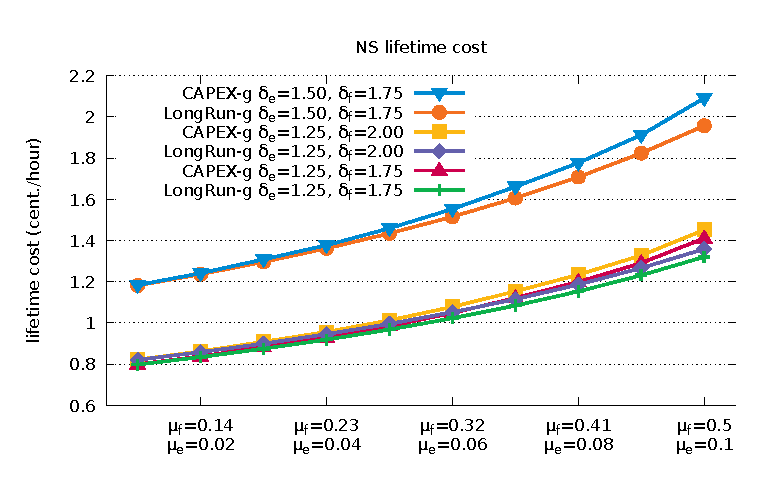
\includegraphics[width=0.8\textwidth]{img/lifecost.eps}
        \caption{Evaluation on VNE on top of \textbf{5GEN} graph}
    \end{figure}
\end{frame}



\section{Conclusions}
\begin{frame}{Advantages}
    \begin{itemize}
        \item stores the graph as GML (easy to parse);
        \item Arbitrarily big graphs;
        \item SDNlib has small reference abstracted graphs;
        \item it is based on ITU \cite{itu};
        \item open source: \url{https://github.com/MartinPJorge/mec-generator/tree/5g-infra-gen}; and
        \item Given the AAUs it creates the whole infrastructure.
    \end{itemize}
\end{frame}


\begin{frame}{References}
    \bibliographystyle{IEEEtran}
    \bibliography{bibliography}
\end{frame}


\end{document}
